%DOCUMENT NAME: 8086 Microprocessor Cheatsheet, TexStudio
%AUTHOR NAME: Jishan Shaikh
%LAST UPDATED: November 6, 2018
%v2: May 28, 2022


\documentclass[12pt, a4paper]{scrartcl}

\usepackage
[
	a4paper,
	outer=1.5cm,
	inner=1.5cm,
	top=1.75cm,
	bottom=1.5cm
]{geometry}

%\twocolumn

\usepackage{graphicx}
\usepackage
[	colorlinks,
	linkcolor={blue},
	citecolor={blue},
	urlcolor={blue}		
]{hyperref}

%opening
\title{8086 Microprocessor Cheatsheet}

\author{Jishan Shaikh\footnote{v2 (2022) with updated descriptions, proofread, and erratas. Compiled during CSE-313 (Microprocessors) and CSE-316 (Microprocessors Lab) at National Institute of Technology, Bhopal (India). \textbf{MIT License.}\\
		.}\\{\normalsize  \href{mailto:jishanshaikh9893@gmail.com}{jishanshaikh9893@gmail.com}}}
\date{May 28, 2022}

\begin{document}

\maketitle

\begin{abstract}
	\textbf{Abstract:} This cheat sheet contains information about the 8086 microprocessors. Compared to standard textbooks, the main focus is conciseness, to-the-point descriptions, and readability. It is a direct result of scribe notes taken for the subject -- microprocessors (3+1 credits). The main topics included in the document are 8086 overviews, internal architecture, register organization, modes of operation, addressing modes, interrupts, memory, and assembly language programs (Instruction types, Memory segmentation, and Memory models). The program bank contains an excellent collection of ASM program questions. A question bank is also provided for examinations/quizzes. This cheat sheet is published as an open document at \href{https://www.github.com/jishanshaikh4/8086-cheatsheet/}{www.github.com/jishanshaikh4/8086-cheatsheet/}. You are more than welcome to use this! 
\end{abstract}

\section{8086 Overview}
	8086 is a 16-bit microprocessor. It has a 20-bit address bus that can access up to $2^{20}$ memory locations (1 MB). It can support up to 64K input/output ports. It provides 14, 16-bit internal registers. It has multiplexed address and data bus $AD_{0}-AD_{15}$ and $A_{16}-A_{19}$. It requires a single-phase clock with a 33\% duty cycle to provide an internal cycle. It has two operation modes - Minimum and Maximum mode. Its improvements over the 8085 microprocessors include pipelining, instruction queue, and segmentation. It can pre-fetch up to 6 instruction bytes from memory and queue them to speed up instruction execution (Pipelining). It usually requires a +5V power supply. It is packaged under a 40-pin dual inlined package.

\section{Internal Architecture}
	8086 has two blocks, BIU (Bus Interface Unit) and EU (Execution Unit). The BIU performs all bus operations such as instruction fetching, reading, and writing operands to memory and calculating the address of memory operands. The instruction bytes are transferred to the instruction queue. EU executes instructions from the instruction system byte queue. Both units operate asynchronously to give the 8086 an overlapping instruction fetch and execution mechanism, called Pipelining. This results in efficient use of system bus and system performance. BIU contains an Instruction queue, Segment registers, Instruction pointer, and Address adder. EU contains Control circuitry, Instruction decoder, ALU, Pointer and index register, and Flag register. 	\\
	
	\begin{figure}[h]
		\centering
		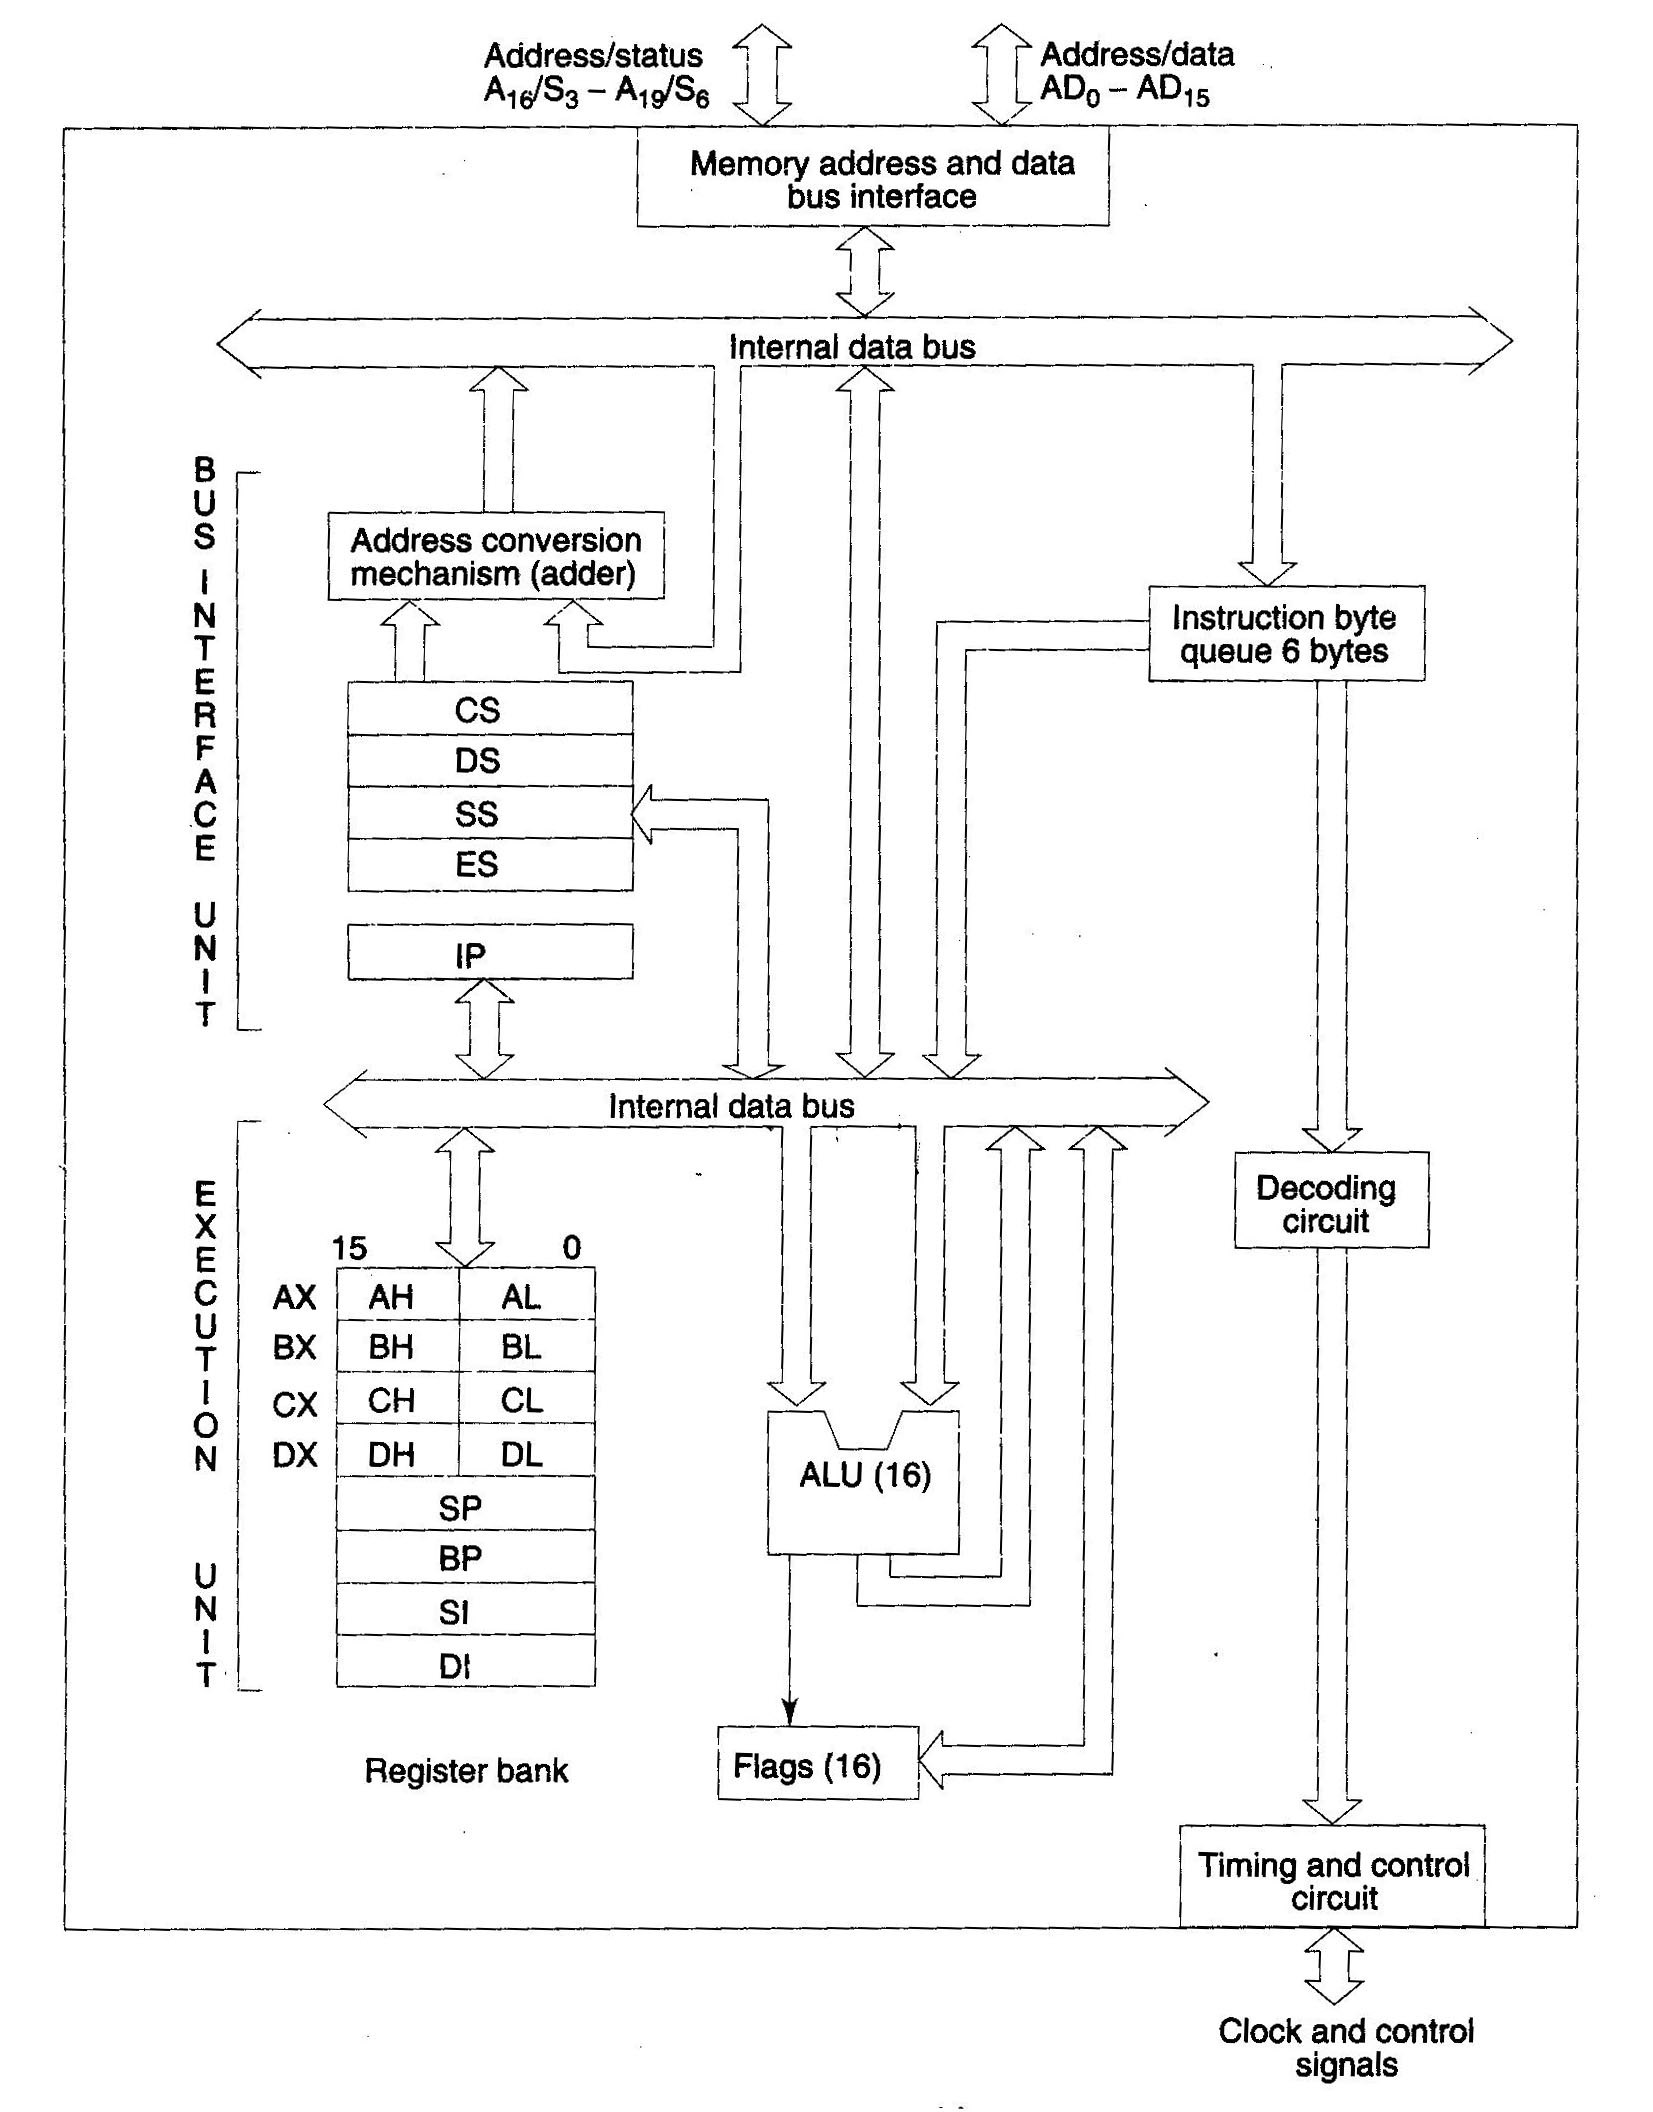
\includegraphics[width=0.75\textwidth]{images/8086-architecture.png}
		\caption{8086 Architecture diagram.}
		\label{image-1}
	\end{figure}
	
	\textbf{Bus Interface Unit (BIU): }It provides a full 16-bit bidirectional data bus and 20-bit address bus, and is fully responsible for performing all external bus operations. The functions of BIU include instruction fetch, instruction queuing, operand fetch, storage, address relocation, and bus control. It uses a mechanism known as an instruction stream queue to implement a pipeline architecture. This queue permits the prefetch of up to 6 bytes of instruction code. Prefetching instructions are held in its FIFO queue.
	
	\begin{figure}[h]
		\centering
		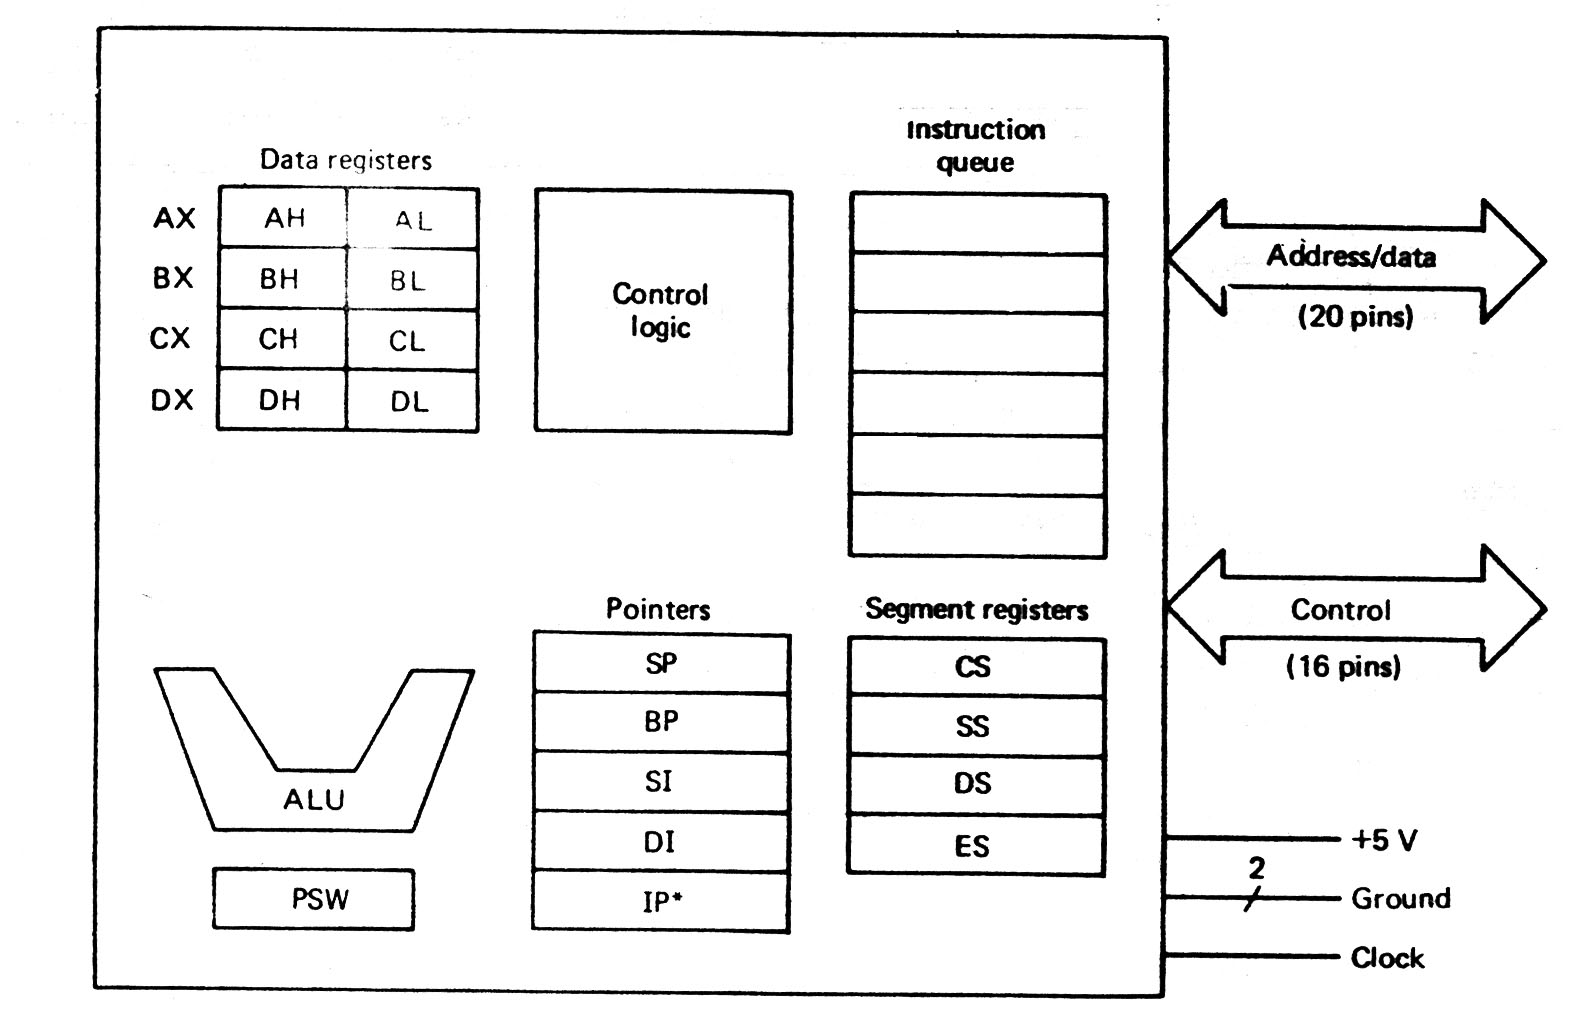
\includegraphics[width=0.89\textwidth]{images/8086-internal-bus-configuration.png}
		\caption{8086 Internal bus configuration.}
		\label{image-2}
	\end{figure}
	
	Since the data bus is of 16-bit size, BIU can fetch two instruction bytes in a single memory cycle. The time interval of which there doesn't any bus activity is known as \textit{Idle state}, which may occur between bus cycles. The BIU also contains a dedicated adder, which is used to generate a 20-bit physical address that is the output of the address bus. It is formed by adding an appended 16-bit segment address and a 16-bit offset address. BIU is also responsible for the generation of bus control signals, such as those of memory read or write and I/O read or write. \\
	
	\textbf{Execution Unit (EU): }It handles decoding and executing all instructions. The EU extracts instructions from the top of the queue in the BIU, decodes them, generates operands if necessary, passes them to the BIU, and requests it to perform the read or write bus cycles to memory or I/O and perform the operation specified by the instruction on the operands. During the execution of the instruction, the EU tests the status and control flags and updates them based on the results of executing the instruction. If the queue is empty, the EU has to wait for the next instruction byte to be fetched and shifted to the top of the queue. When the EU executes a branch or jump instruction, it transfers control to a location corresponding to another set of sequential instructions. Whenever this happens, the BIU resets the queue and then begins to fetch instructions from this new location to refill the queue.

	\begin{figure}[h]
		\centering
		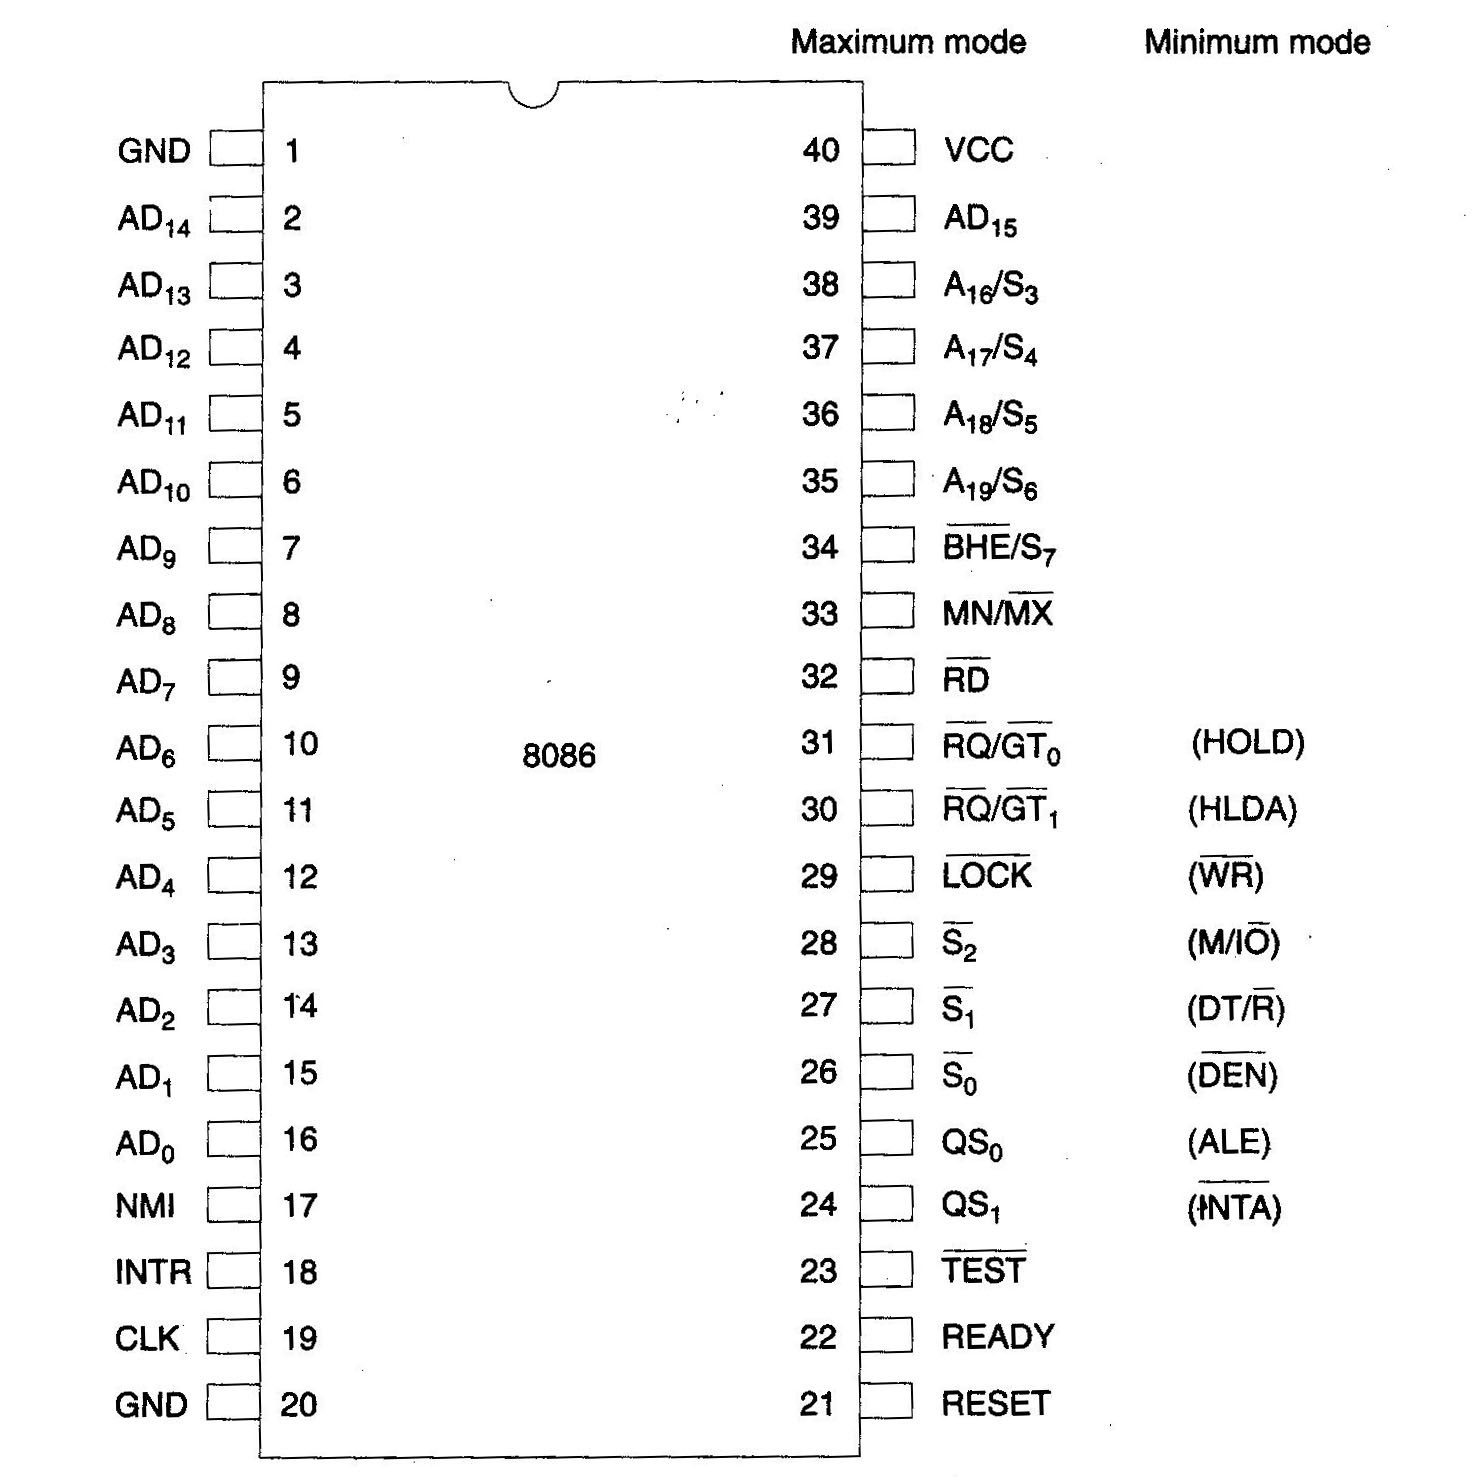
\includegraphics[width=0.65\textwidth]{images/8086-pin-configuration.png}
		\caption{8086 Pin configuration.}
		\label{image-3}
	\end{figure}

\section{Register organization}
	The 8086 has four groups of user-accessible internal registers. They are instruction pointer, four data registers, four-pointer and index register, and four segment registers. 8086 has a total of 14, 16-bit registers including a 16-bit register called \textit{status register}, with 9-bits implemented for status and control flags. Most of the registers contain data/instruction offsets within the 64 KB memory segment. There are four different 64 KB segments for instructions, stack, data, and extra data. To specify where in 1 MB of processor memory these 4 segments are located, the processor uses \textbf{four segment registers:} \\
	
	\textbf{Code Segment (CS): }It is a 16-bit register containing the address of a 64-bit segment with processor instructions. The
	processor uses CS segment for all accesses to instructions
	referenced by instruction pointer (IP) register. CS register
	cannot be changed directly. The CS register is automatically updated during far jump, far call and far
	return instructions. \\
	
	\textbf{Stack Segment (SS): }It is a 16-bit register containing address of 64 KB segment with program stack. By default, the
	processor assumes that all data referenced by the stack	pointer (SP) and base pointer (BP) registers is located in
	the stack segment. SS register can be changed directly using POP instruction. \\
	
	\textbf{Data Segment (DS): }It is a 16-bit register containing address	of 64 KB segment with program data. By default, the
	processor assumes that all data referenced by general registers (AX, BX, CX, DX) and index register (SI, DI) is located in the data segment. DS register can be changed	directly using POP and LDS instructions. \\
	
	\textbf{Extra Segment (ES): }It is a 16-bit register containing address of 64 KB segment, usually with program data. By default,
	the processor assumes that the DI register references the
	ES segment in string manipulation instructions. ES register
	can be changed directly using POP and LES instructions. \\
	
	It is possible to change default segments used by general
	and index registers by prefixing instructions with a CS, SS,
	DS or ES prefix. All general registers of the 8086 microprocessor can be used for arithmetic and logic operations. \textbf{The general
		registers} are: \\
	
	\textbf{Accumulator: }register consists of two 8-bit registers AL and AH, which can be combined and used as a 16-bit register AX. AL in this case contains the low-order byte
	of the word, and AH contains the high-order byte.
	Accumulator can be used for I/O operations and string
	manipulation. \\
	
	\textbf{Base: }register consists of two 8-bit registers BL and BH,
	which can be combined and used as a 16-bit
	register BX. BL in this case contains the low-order byte of
	the word and BH contains the high-order byte. BX register
	usually contains a data pointer used for based, based
	indexed or register indirect addressing. \\
	
	\textbf{Count: }register consists of two 8-bit registers CL and CH,
	which can be combined and used as a 16-bit
	register CX. When combined, the CL register contains the
	low-order byte of the word, and CH contains the high-order byte. Count register can be used in Loop, shift/rotate
	instructions and as a counter in string manipulation. \\
	
	\textbf{Data: }register consists of two 8-bit registers DL and DH,	which can be combined and used as a 16-bit
	register DX. When combined, the DL register contains the
	low-order byte of the word, and DH contains the high-order byte. Data register can be used as a port number in
	I/O operations. In integer 32-bit multiply and divide
	instruction the DX register contains the high-order word of the
	initial or resulting number. \\
	
	The following registers are both \textbf{general and index registers}:\\
	
	\textbf{Stack Pointer (SP): }It is a 16-bit register pointing to the program stack. \\
	
	\textbf{Base Pointer (BP): }It is a 16-bit register pointing to data in stack segment. BP register is usually used for based, based indexed, or register indirect addressing. \\
	
	\textbf{Source Index (SI): }It is a 16-bit register used for indexed, based indexed, and register indirect addressing, as well as a source data address in string manipulation instructions.\\ 
	
	\textbf{Destination Index (DI): }It is a 16-bit register used for indexed, based indexed, and register indirect addressing, as well as a destination data addressing in string manipulation instructions.\\
	
	Other registers include \textbf{Instruction Pointer (IP)} and \textbf{Flag register} both of which are of 16-bit size. Only 9-bits of Flag register are used for setting flag bits (Other bits are don't care bits and useless in context), and are as follows: \\
	
	\begin{figure}[h]
		\centering
		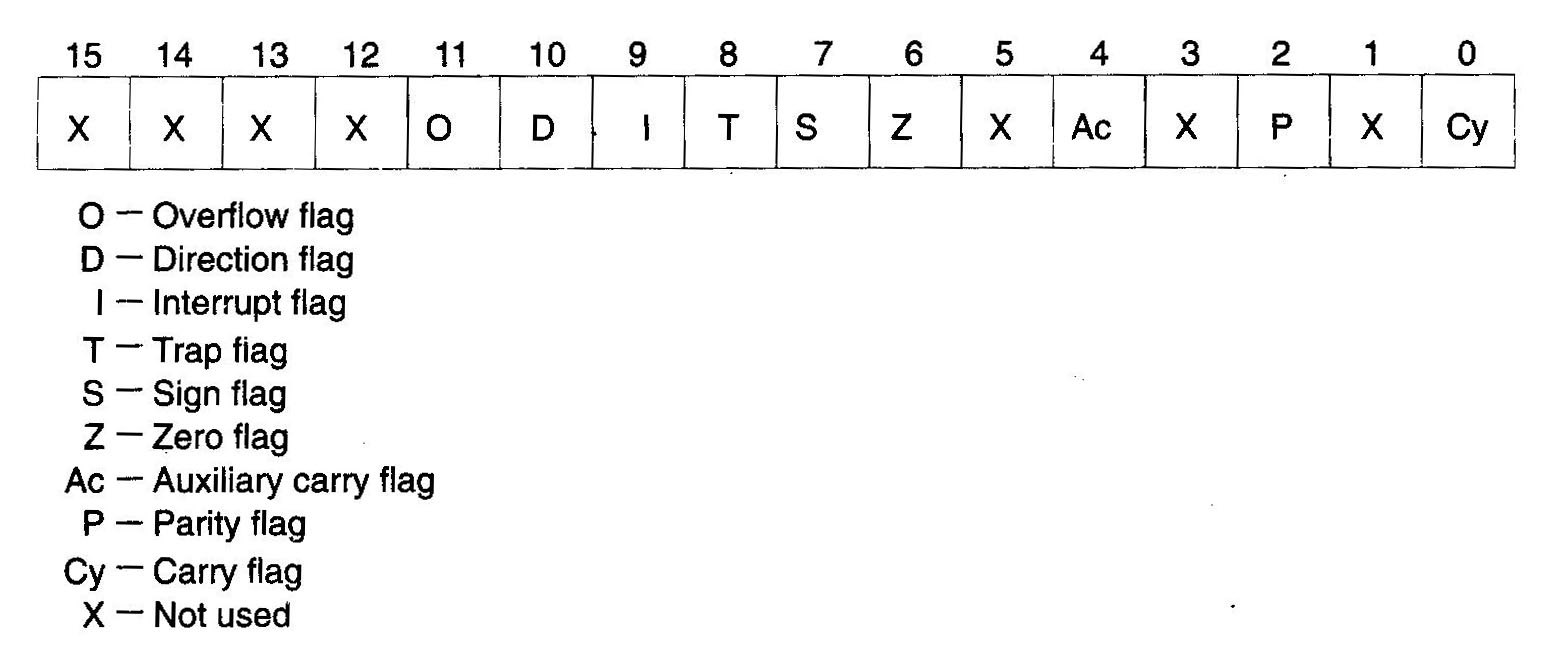
\includegraphics[width=0.89\textwidth]{images/8086-flag-registers.png}
		\caption{8086 Flag register.}
		\label{image-4}
	\end{figure}
	
	\textbf{Overflow Flag (OF): }Set if the result is a too large positive number or is a too small negative number to fit into the destination operand. \\
	
	\textbf{Destination Flag (DF): }If set, then string manipulation instructions will auto-decrement index registers. If cleared, then the index registers will be auto-incremented. \\
	
	\textbf{Interrupt-enable Flag (IF): }Setting this bit enables maskable interrupts. \\
	
	\textbf{Single-step Flag (TF): }If set, then a single-step interrupt will occur after the next instruction. \\
	
	\textbf{Sign Flag (SF): }Set if the most significant bit of the result is set. \\
	
	\textbf{Zero Flag (ZF): }Set if the result is zero (not set). \\
	
	\textbf{Auxiliary carry Flag (AF): }Set if there was a carry from or borrow to bits 0-3 in the AL register. \\
	
	\textbf{Parity Flag (PF): }Set if the parity (the number of 1s) in the lower order byte of the result is even. \\
	
	\textbf{Carry Flag (CF): }Set if there was a carry from or borrow to the most significant bit during the last result calculation.\\
	
\section{Modes of operation: Minimum and Maximum mode}

	\textbf{Minimum mode: }The minimum mode is selected by applying logic 1 to the MN/MX\# input pin. This is a single microprocessor configuration. See figures 5 and 6 of Memory read and write timing diagrams of 8086 in minimum mode.\\
	
	\begin{figure}[h]
		\centering
		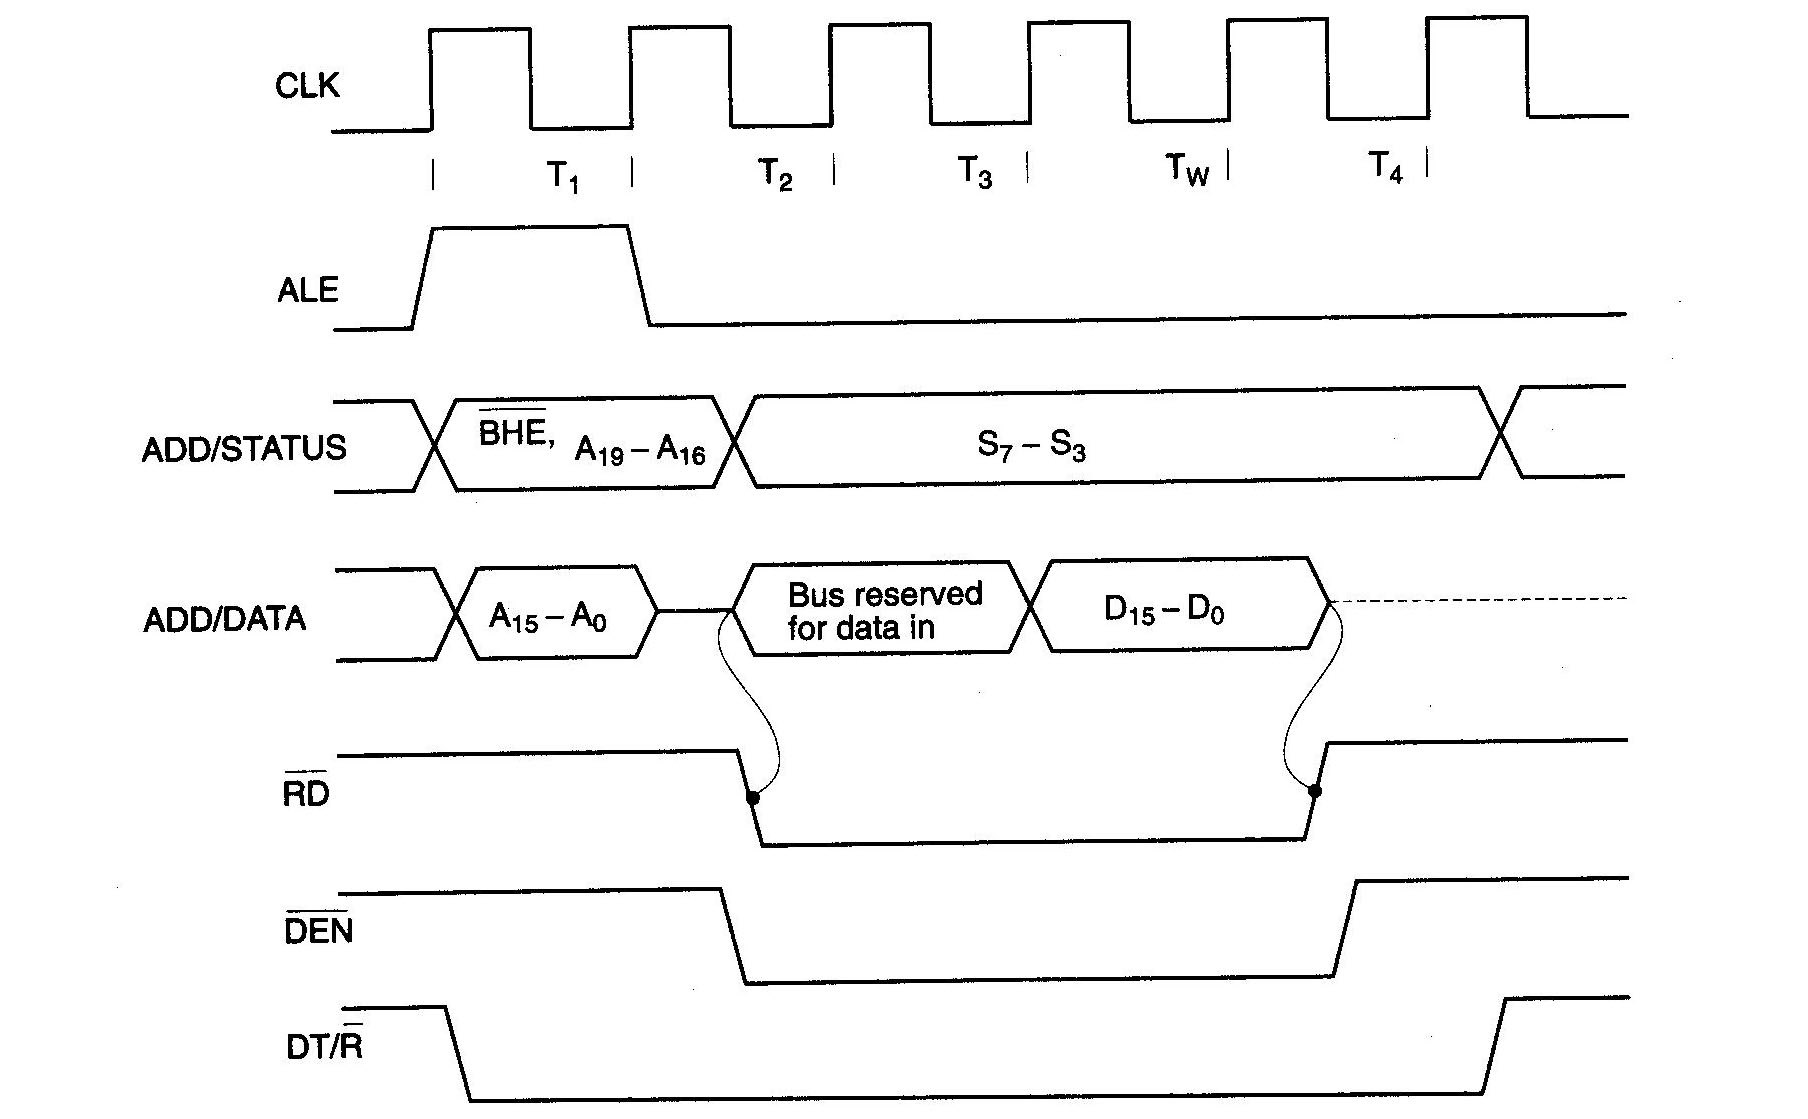
\includegraphics[width=0.75\textwidth]{images/8086-min-read.png}
		\caption{8086 Memory read timing diagram in minimum mode.}
		\label{image-5}
	\end{figure}

	\begin{figure}[h]
		\centering
		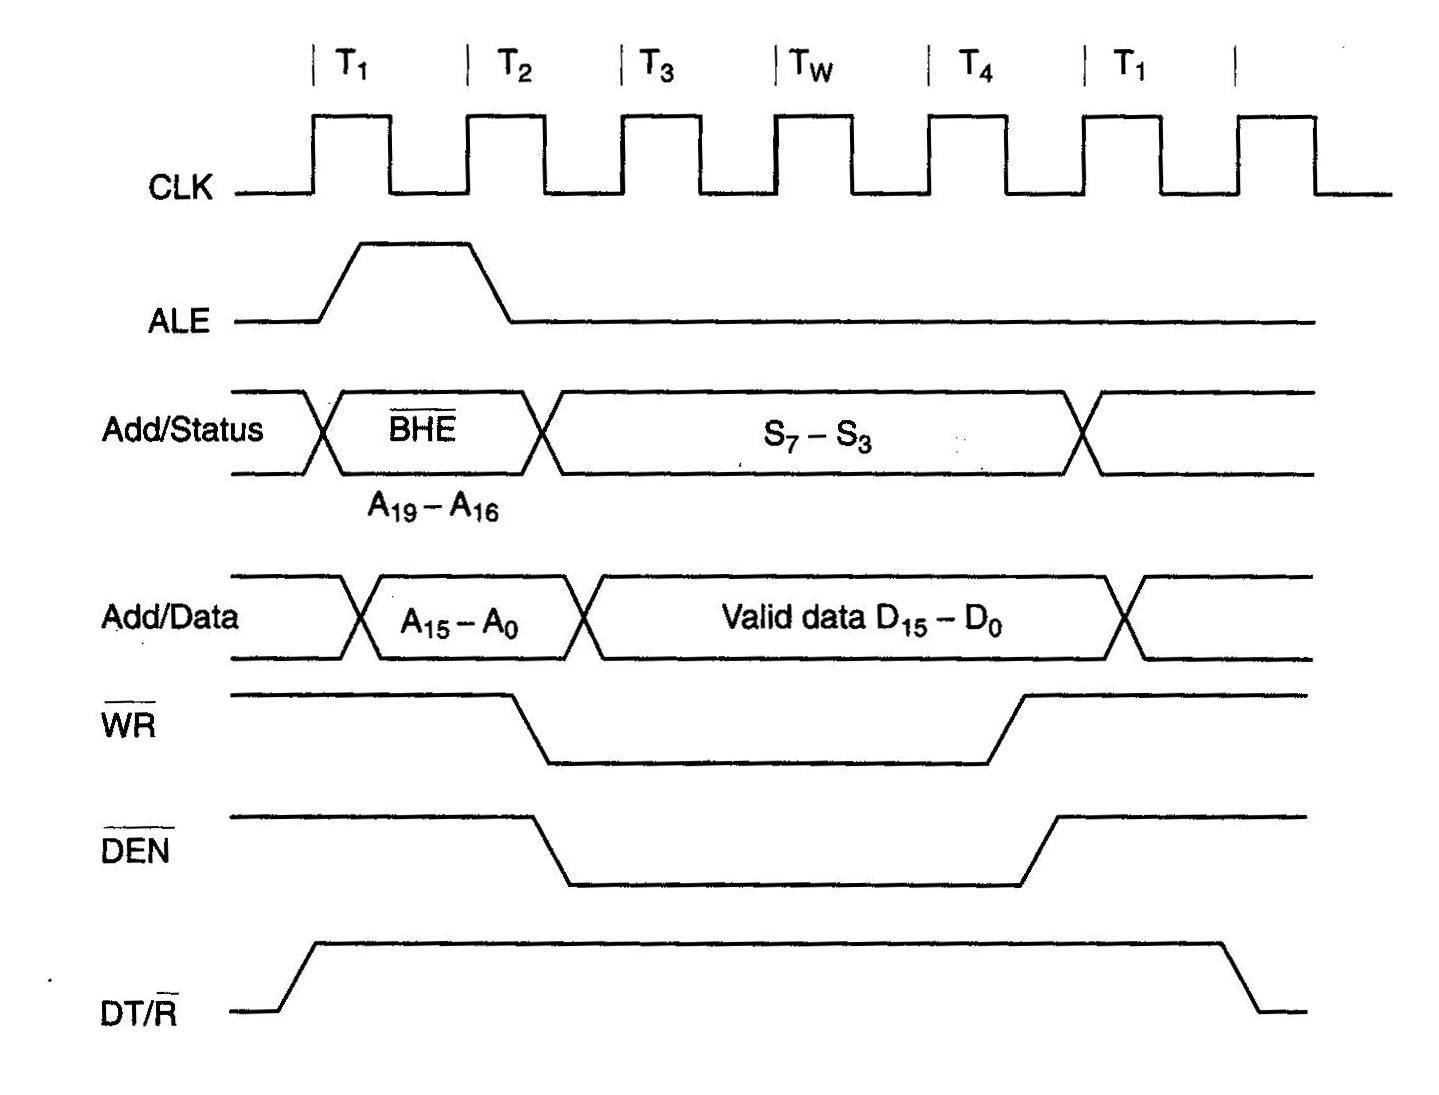
\includegraphics[width=0.75\textwidth]{images/8086-min-write.png}
		\caption{8086 Memory write timing diagram in minimum mode.}
		\label{image-6}
	\end{figure}
	
	\textbf{Maximum mode: }The maximum mode is selected by applying logic 0 to the MN/MX\# input pin. This is a multi microprocessor configuration. See figures 7 and 8 of Memory read and write timing diagrams of 8086 in maximum mode.

	\begin{figure}[h]
		\centering
		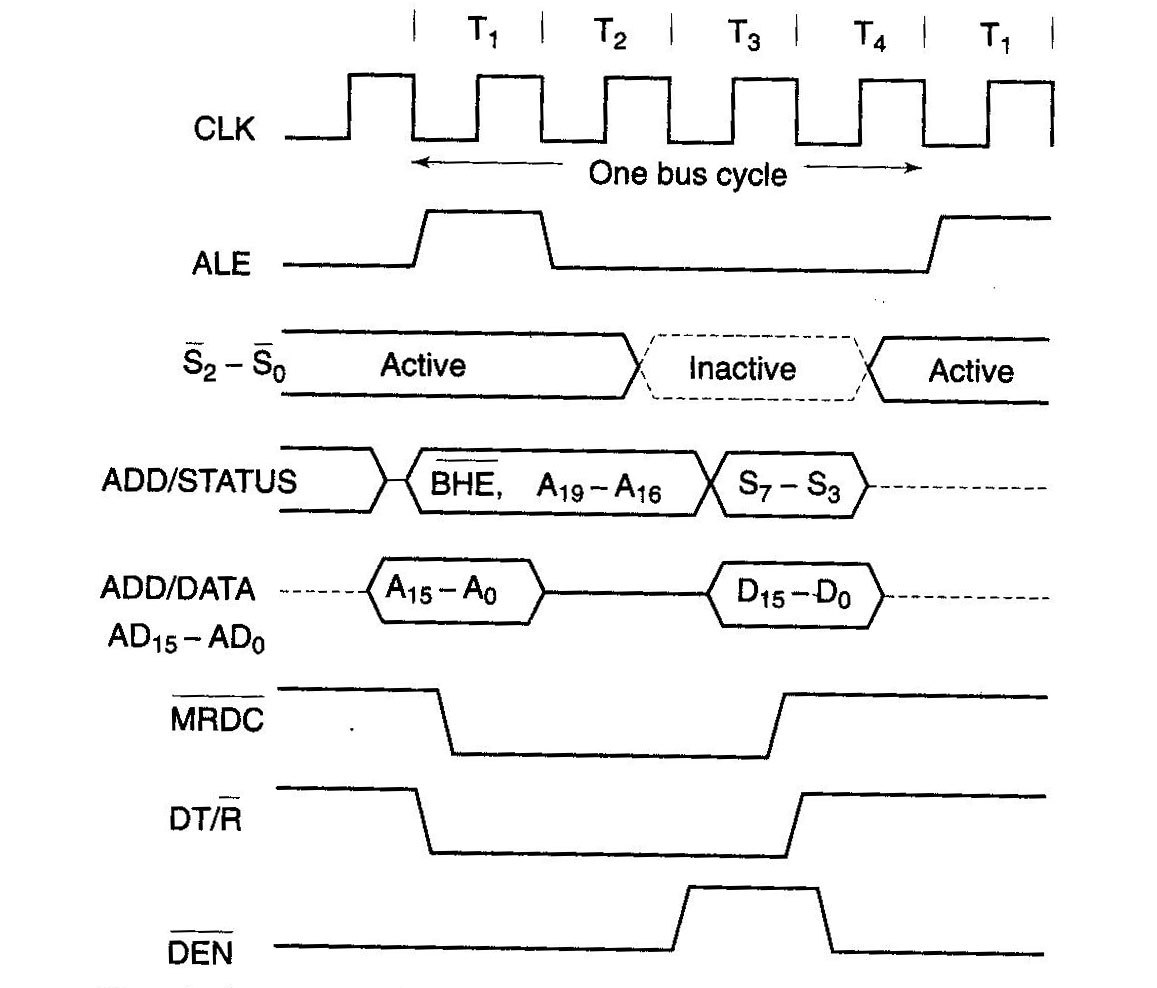
\includegraphics[width=0.75\textwidth]{images/8086-max-read.png}
		\caption{8086 Memory read timing diagram in maximum mode.}
		\label{image-7}
	\end{figure}

	\begin{figure}[h]
		\centering
		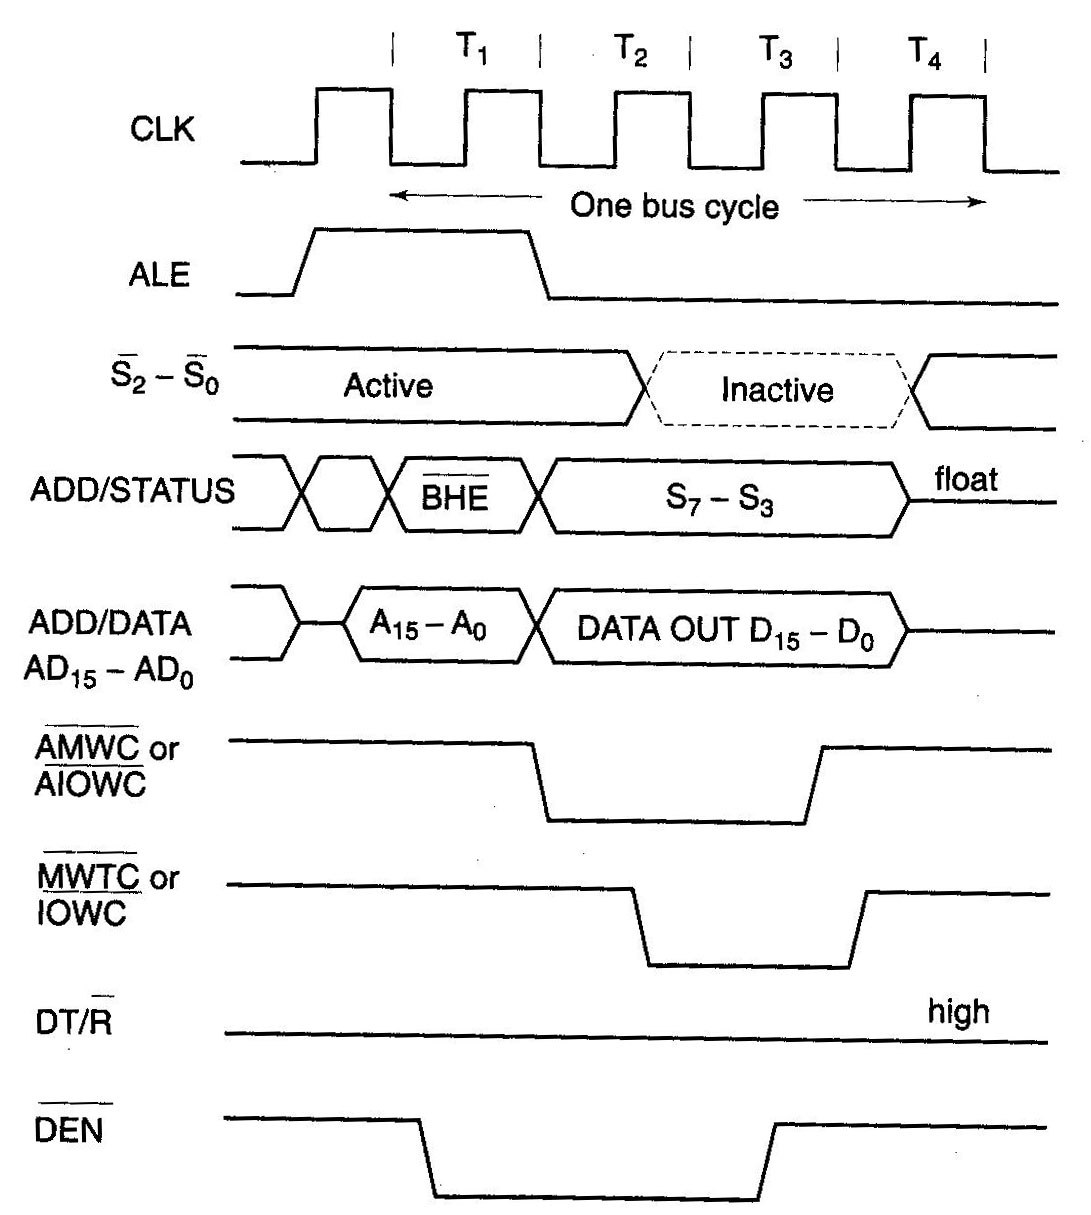
\includegraphics[width=0.75\textwidth]{images/8086-max-write.png}
		\caption{8086 Memory write timing diagram in maximum mode.}
		\label{image-8}
	\end{figure}
	
\section{Addressing Modes}
	The addressing modes supported by 8086 are-\\
	
	\textbf{Implied: }The data value/data address is implicitly associated with the instruction. \\
	
	\textbf{Register: }References the data in a register or in a register pair. \\
	
	\textbf{Immediate: }The data is provided in the instruction.\\
	
	\textbf{Direct: }The instruction operand satisfies the memory address where data is located (Memory direct). \\
	
	\textbf{Register Indirect: }The instruction specifies a register containing an address, where data is located. This addressing mode works with SI, DI, BX, and BP registers.\\
	
	\textbf{Based: }8-bit or 16-bit instruction operand is added to the contents of a base register (BX or BP), and the resulting value is a pointer to the location where data resides. \\
	
	\textbf{Indexed: }8-bit or 16-bit instruction operand is added to the contents of an index register (SI or DI), and the resulting value is a pointer to the location where data resides. \\
	
	\textbf{Based Indexed: }The contents of a base register (BX or BP) is added to the contents of an index register (SI or DI), and the resulting value is a pointer to the location where data resides. \\
	
	\textbf{Based Indexed with displacement: }8-bit or 16-bit instruction operand is added to the contents of a base register (BX or BP) and index register (SI or DI), the resulting value is a pointer to the location where data resides.\\

\section{Interrupts}
	\textbf{Execution sequence for handling an interrupt: }When an interrupt occurs, the processor stores a FLAGS register into a stack, disables further interrupts, fetches from the bus one byte representing interrupt type, and jumps to interrupt processing routine, the address of which is stored in location 4 * interrupt\_type\_address. The interrupt processing routine should return with the IRET instruction. \\
	
	8086 has the following interrupts-\\
	
	\textbf{INTR: }It is a maskable hardware interrupt. The interrupt can be enabled/disabled using STI/CLI instructions or using more complicated method of updating the FLAGS register with the help of the POPF instruction.\\
	
	\textbf{NMI: }It is a non-maskable interrupt. The interrupt is processed in the same way as the INTR interrupt. Interrupt type of the NMI is 2, i.e. the address of the NMI processing routine is stored in location 0008h. This interrupt has higher priority than the maskable interrupt.\\
	
	\textbf{Software Interrupts: }can be caused by: \\
	
	\textbf{INT instruction: }Breakpoint interrupt. This is a type-3 interrupt.\\
	
	\textbf{INT interrupt\_number instruction: }Any one of interrupt from available 256 interrupts. \\
	
	\textbf{INTO instruction: }Interrupt on overflow.\\
	
	\textbf{Single step interrupt: }Generated if the TF flag is set. This is a type 1 interrupt. When the CPU processes this interrupt, it clears the TF flag before calling the interrupt processing routine. \\
	
	There exists some \textit{processor exceptions} such as divide error (Type 0), Unused opcode (Type 6), and Escape opcode (Type 7). The processing of software interrupts is the same as that of hardware interrupts.

\section{Memory}
	Program, data, and stack memories occupy the same memory space. As the most of the processor instructions use 16-bit pointers, the processor can effectively address only 64 KB of memory. To access memory outside 64 KB, the CPU uses special segment registers to specify where the code, stack and data 64 KB segments are positioned within 1 MB of memory. 16-bit pointers and data are stored as the address: low-order byte, address+1: high-order byte. 32-bit addresses are stored in "segment: offset" format as the address: low-order byte of segment, address+1: high-order byte of segment, address+2: low-order byte of offset, and address+3: high-order byte of offset. Physical memory address pointed by segment: offset pair is calculated as:\\
	
	$$ Physical\ address = (segment\_address * 16) + offset\_address $$\\
	
	\textbf{Program memory: }Program can be located anywhere in memory. Jump and call instructions can be used for short
	jumps within currently selected 64 KB code segment, as
	well as for far jumps anywhere within 1 MB of memory. All conditional jump instructions can be used to jump
	within approximately +127 to -127 bytes from current
	instruction. \\
	
	\textbf{Data memory: }The processor can access data in any one
	out of 4 available segments, which limits the size of
	accessible memory to 256 KB (if all four segments point to
	different 64 KB blocks). Accessing data from the Data, Code, Stack or Extra segments can be usually done by prefixing instructions
	with the DS:, CS:, SS: or ES: (some registers and instructions by default may use the ES or SS segments instead of DS segment). Word data can be located at odd or even byte boundaries.	The processor uses two memory accesses to read a 16-bit	word located at odd byte boundaries. Reading word data from even byte boundaries requires only one memory	access. \\
	
	\textbf{Stack memory: }It can be placed anywhere in memory. The
	stack can be located at odd memory addresses, but it is not
	recommended for performance reasons. \\
	
	0000h-02FFh are reserved memory locations for interrupt vectors. Each interrupt vector is a 32-bit pointer in format segment:offset. FFFF0h-FFFFFh - after reset, the processor always starts program execution at the FFFF0h address.


\section{8086 Assembly Programming}

	\subsection{8086 Instruction types (set)}
	\textbf{Data flow Instructions: }Transfer information between registers and memory locations or I/O ports. e.g. MOV, XCHG, LEA, PUSH, POP, PUSHF, POPF, IN, OUT.\\ 
	\begin{figure}[h]
		\centering
		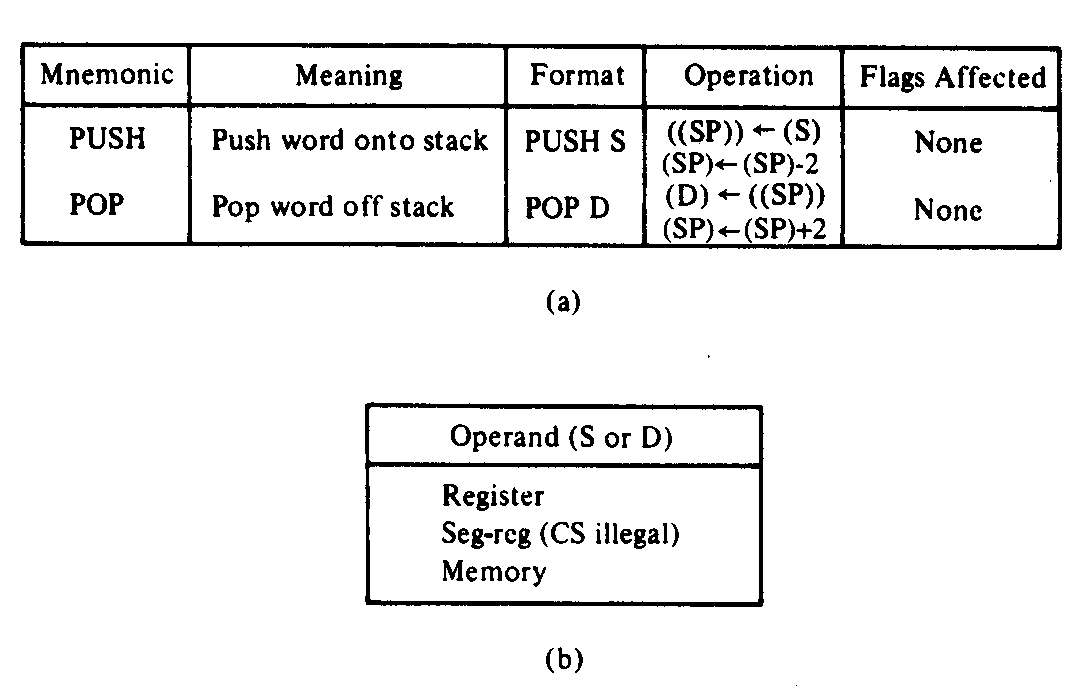
\includegraphics[width=0.95\textwidth]{images/pushpop.png}
		\caption{PUSH and POP instructions.}
		\label{image-9}
	\end{figure}
	\begin{figure}[h]
		\centering
		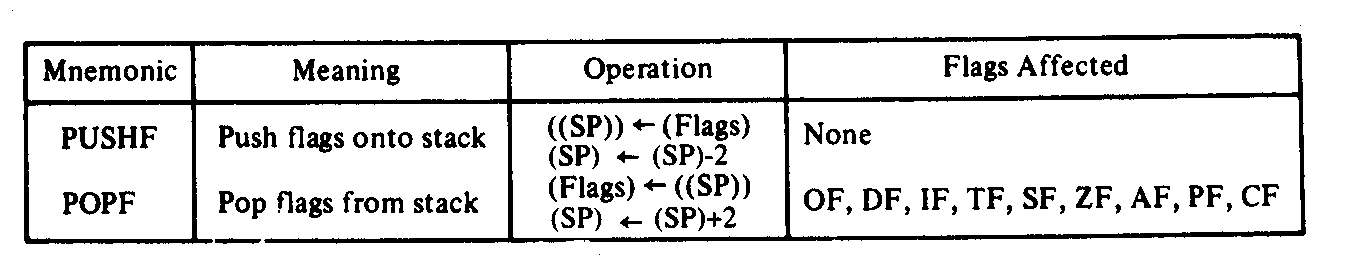
\includegraphics[width=0.95\textwidth]{images/pushfpopf.png}
		\caption{PUSHF and POPF instructions.}
		\label{image-10}
	\end{figure}
	
	\textbf{Arithmetic Instructions: }Perform arithmetic operations on binary or binary-coded-decimal (BCD) numbers. e.g. ADD, SUB, INC, DEC, ADC, SBB, NEG, CMP, MUL, IMUL, DIV, IDIV, CBW, CWD.\\ 
	
	\textbf{Bit manipulation Instructions: }Perform shift, rotate, and logical operations on memory locations and registers. e.g. SHL, SHR, SAR, ROL, ROR, RCL, RCR, NOT, AND, OR, XOR, TEST.\\ 
	
	\textbf{Control transfer (flow) Instructions: }Control sequence of program execution; include jumps and procedure transfers. e.g. JMP, JG, JL, JE, JNE, JGE, JLE, JNG, JNL, JC, JS, JA, JB, JAE, JBE, JNB, JNA, JO, JZ, JNZ, JP, JCXZ, LOOP, LOOPE, LOOPZ, LOOPNE, LOOPNZ, CALL, RET.\\ 
	\begin{figure}[h]
		\centering
		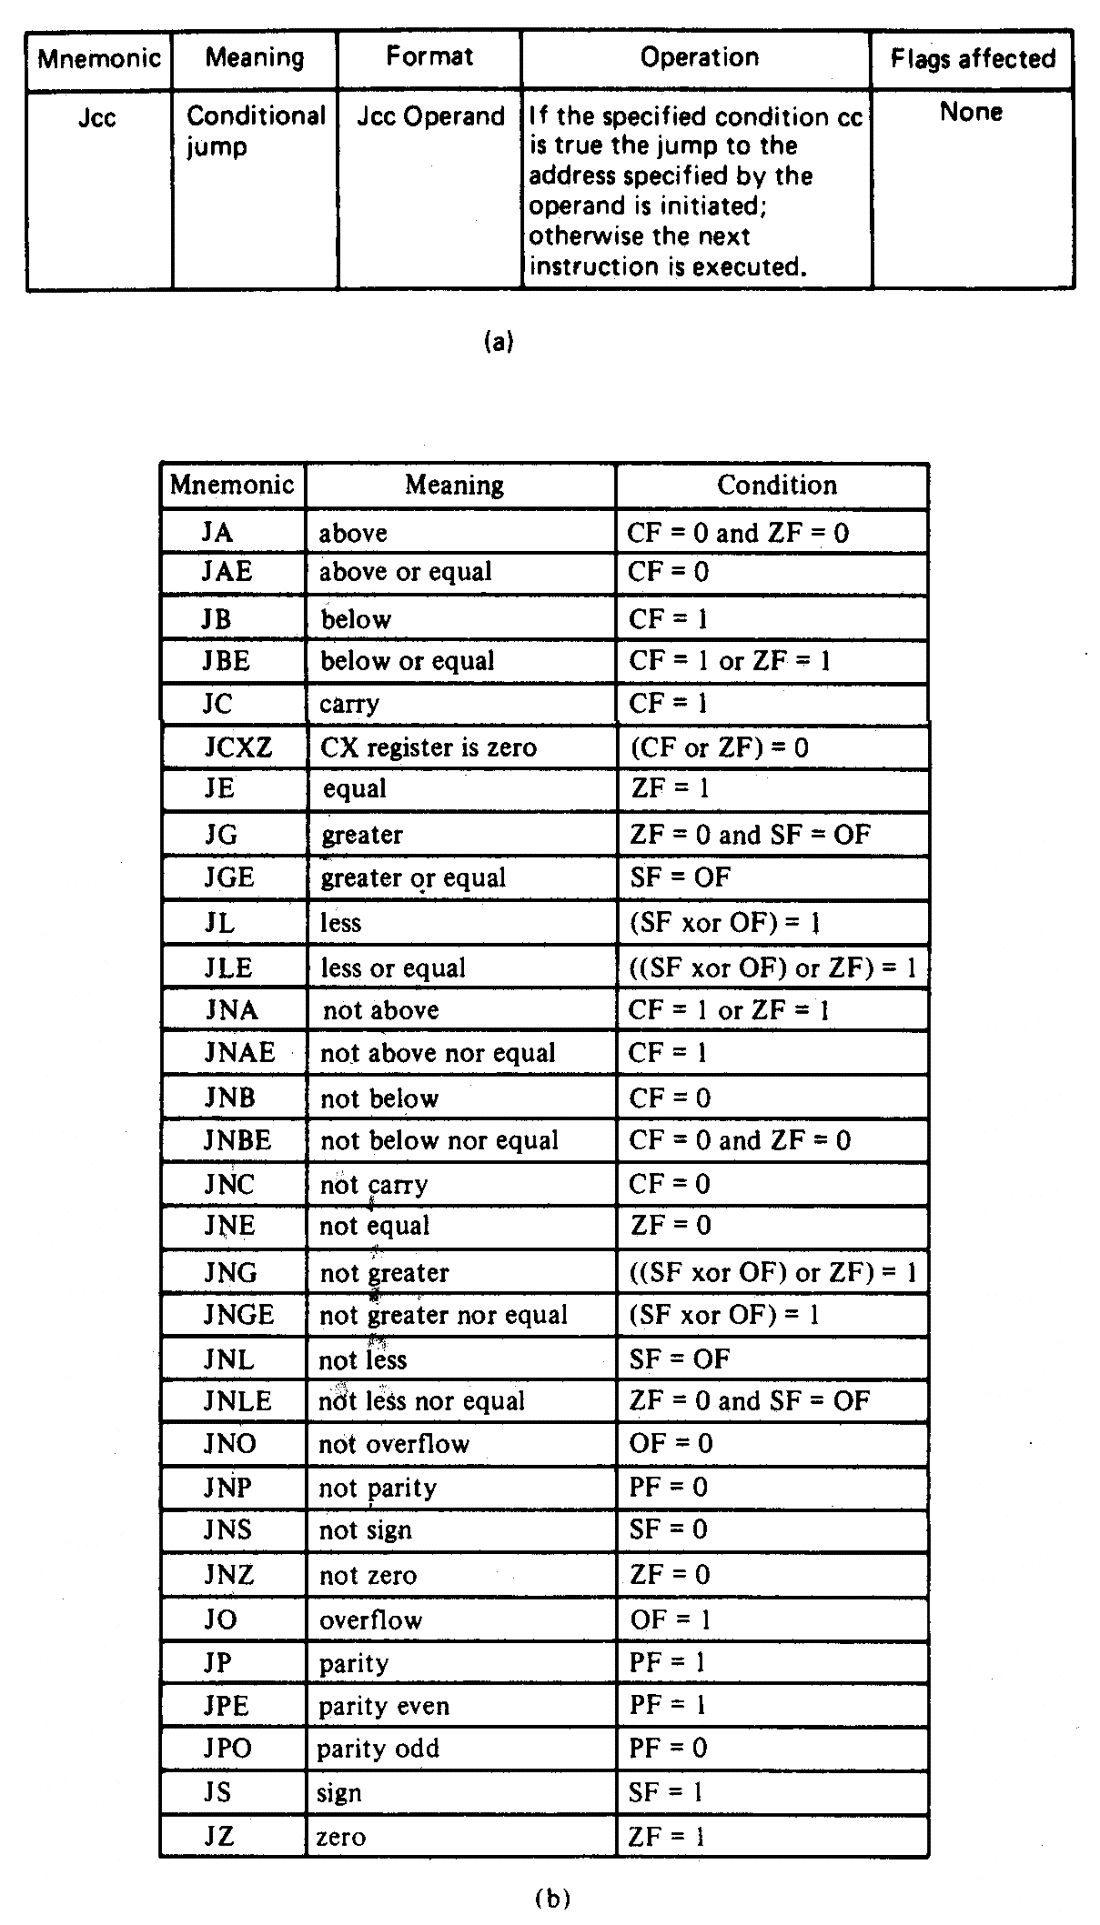
\includegraphics[width=0.65\textwidth]{images/jump.png}
		\caption{Jump instructions.}
		\label{image-11}
	\end{figure}
	\begin{figure}[h]
		\centering
		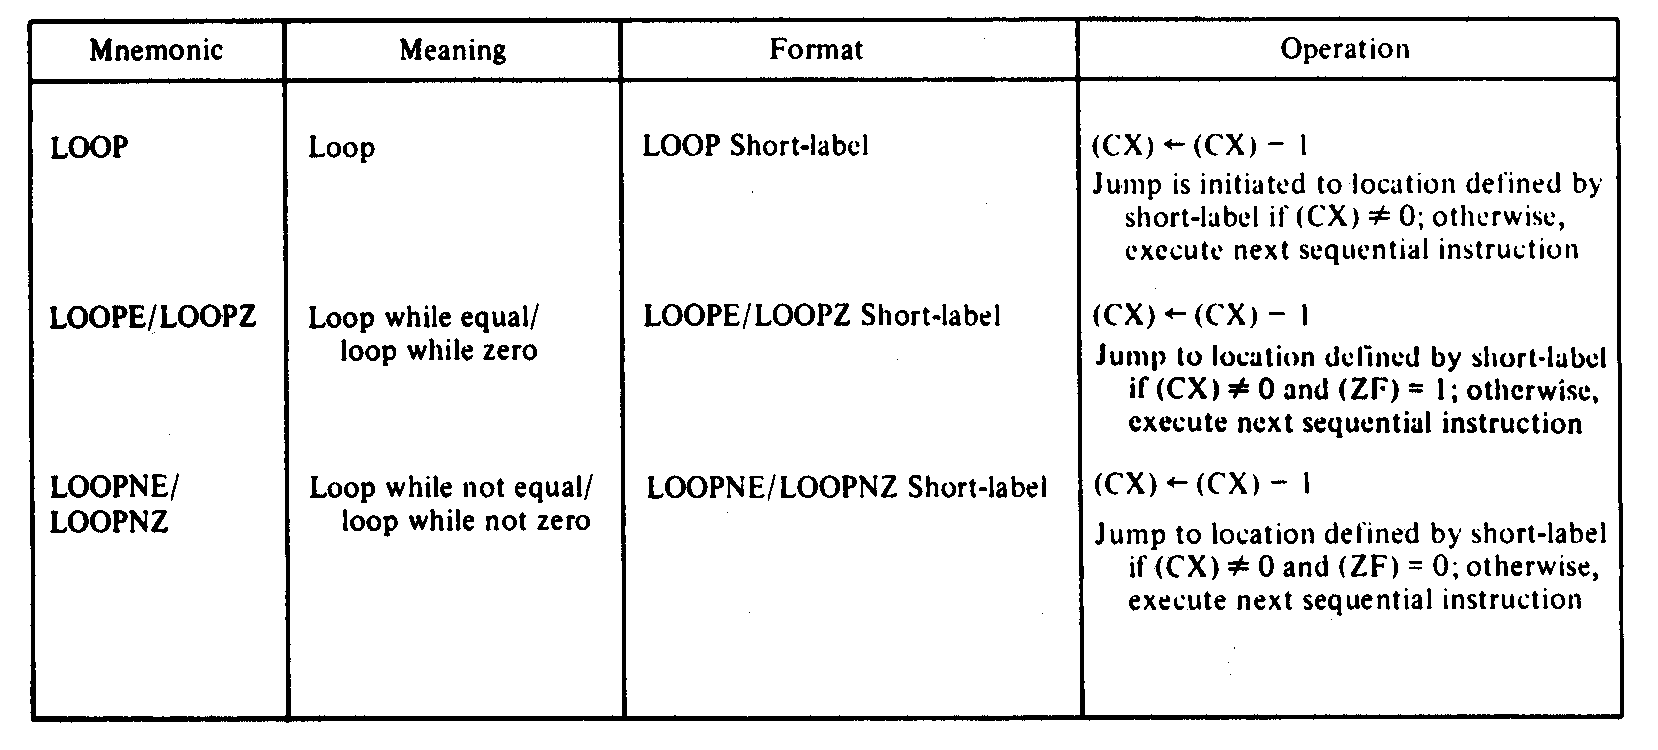
\includegraphics[width=0.9\textwidth]{images/loop.png}
		\caption{Loop instructions.}
		\label{image-12}
	\end{figure}
	
	\textbf{String Instructions: }Move, compare, and scan strings of information. e.g. MOVS, MOVSB, MOVSW, CMPS, CMPSB, CMPSW, SCAS, SCASB, SCASW, LODS, LODSB, LODSW, STOS, STOSB, STOSW.\\ 
	\begin{figure}[h]
		\centering
		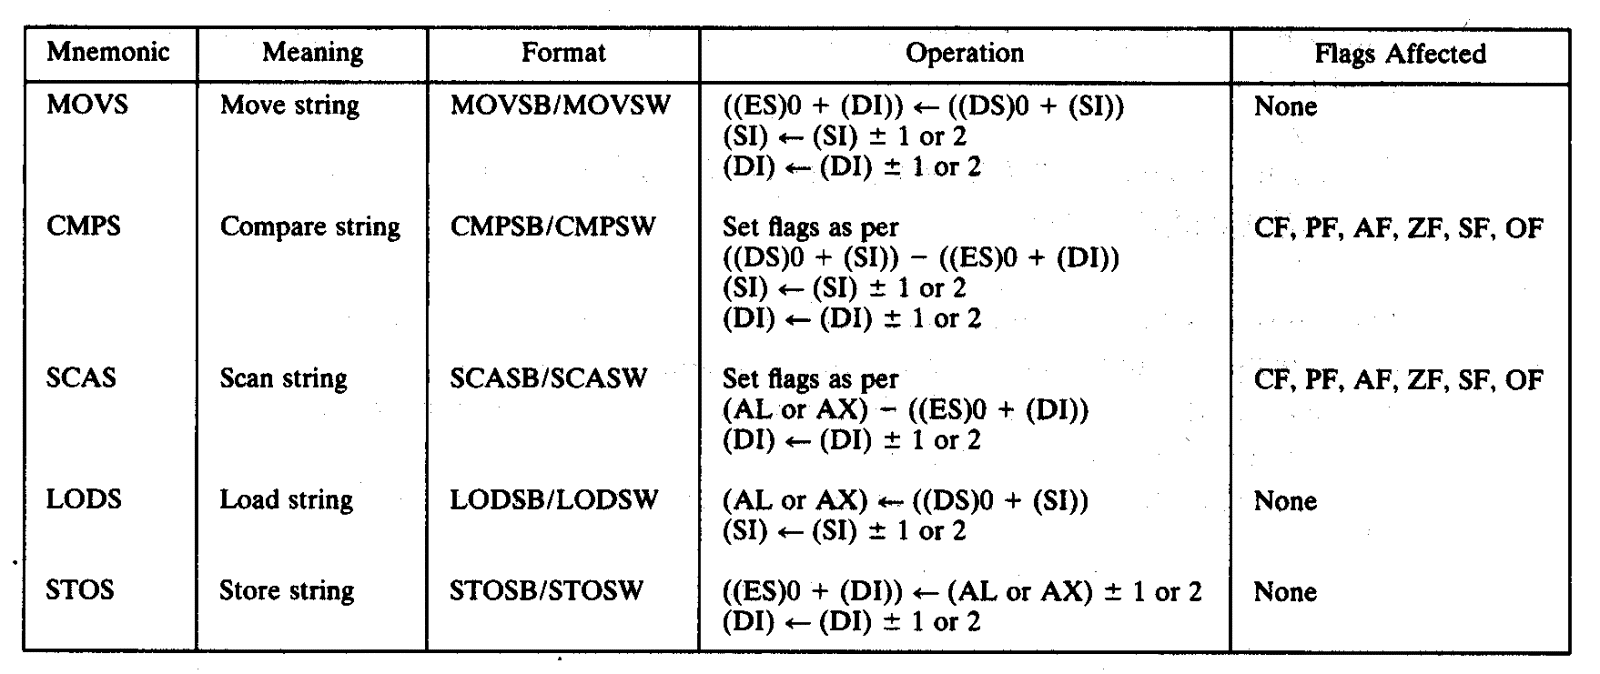
\includegraphics[width=\textwidth]{images/string.png}
		\caption{String handling instructions.}
		\label{image-13}
	\end{figure}
	\begin{figure}[h]
		\centering
		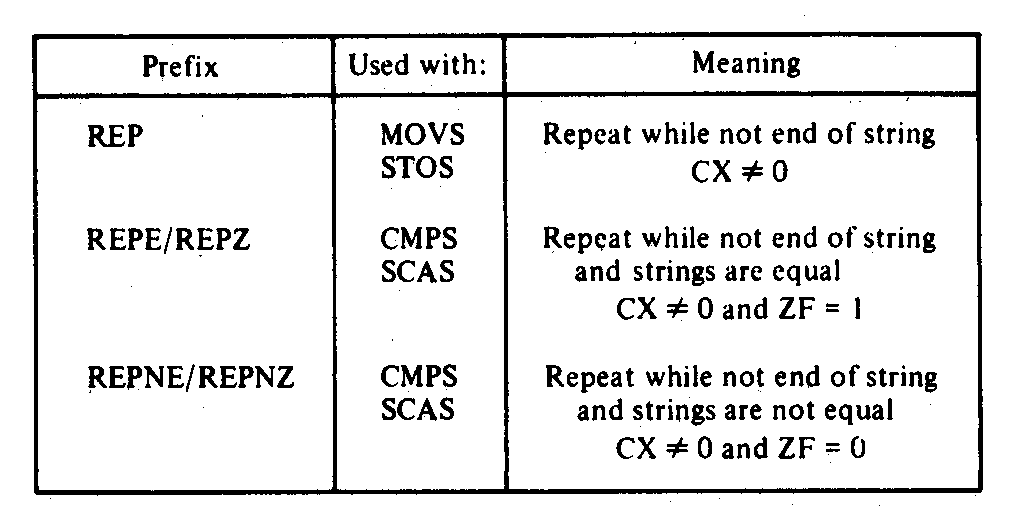
\includegraphics[width=0.8\textwidth]{images/repeat-string.png}
		\caption{Repeat string instructions.}
		\label{image-14}
	\end{figure}
	
	\textbf{Interrupt Instructions: }Interrupt processor to service specific condition. e.g. INT, INTO, IRET.\\ 
	
	\textbf{Processor Control Instructions: }Set and clear status flags, and change the processor execution state, e.g. STC, STD, STI.\\ 
	\begin{figure}[h]
		\centering
		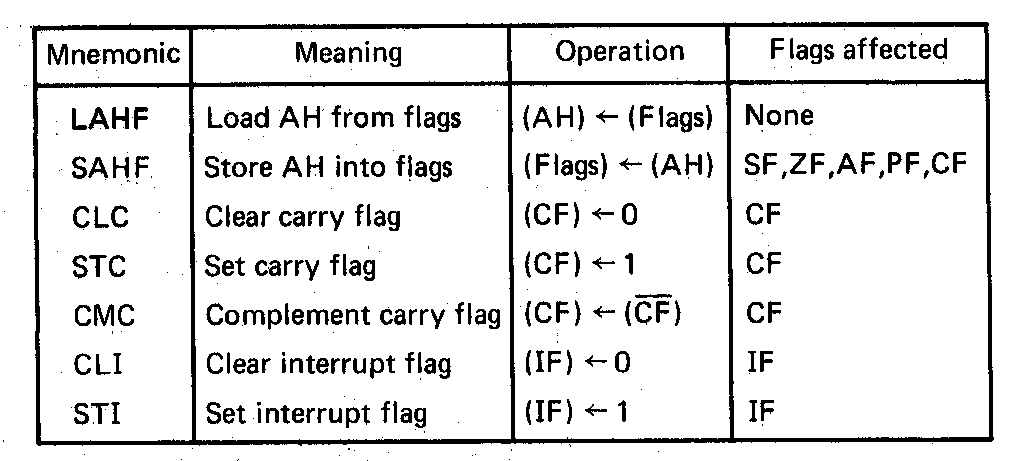
\includegraphics[width=0.9\textwidth]{images/flag.png}
		\caption{Flag (Processor) control instructions.}
		\label{image-15}
	\end{figure}
	
	\textbf{Miscellaneous Instructions: }e.g. NOP, WAIT. 
	
	\subsection{Memory Segmentation} A memory segment is a block of $2^{16}$ (64K) bytes. Each segment is identified by a segment number. Segment number is of 16-bits (0000-FFFF). A memory location is specified by an offset within a segment. Logical address to physical address is discussed in memory section.\\
	
	\begin{figure}[h]
		\centering
		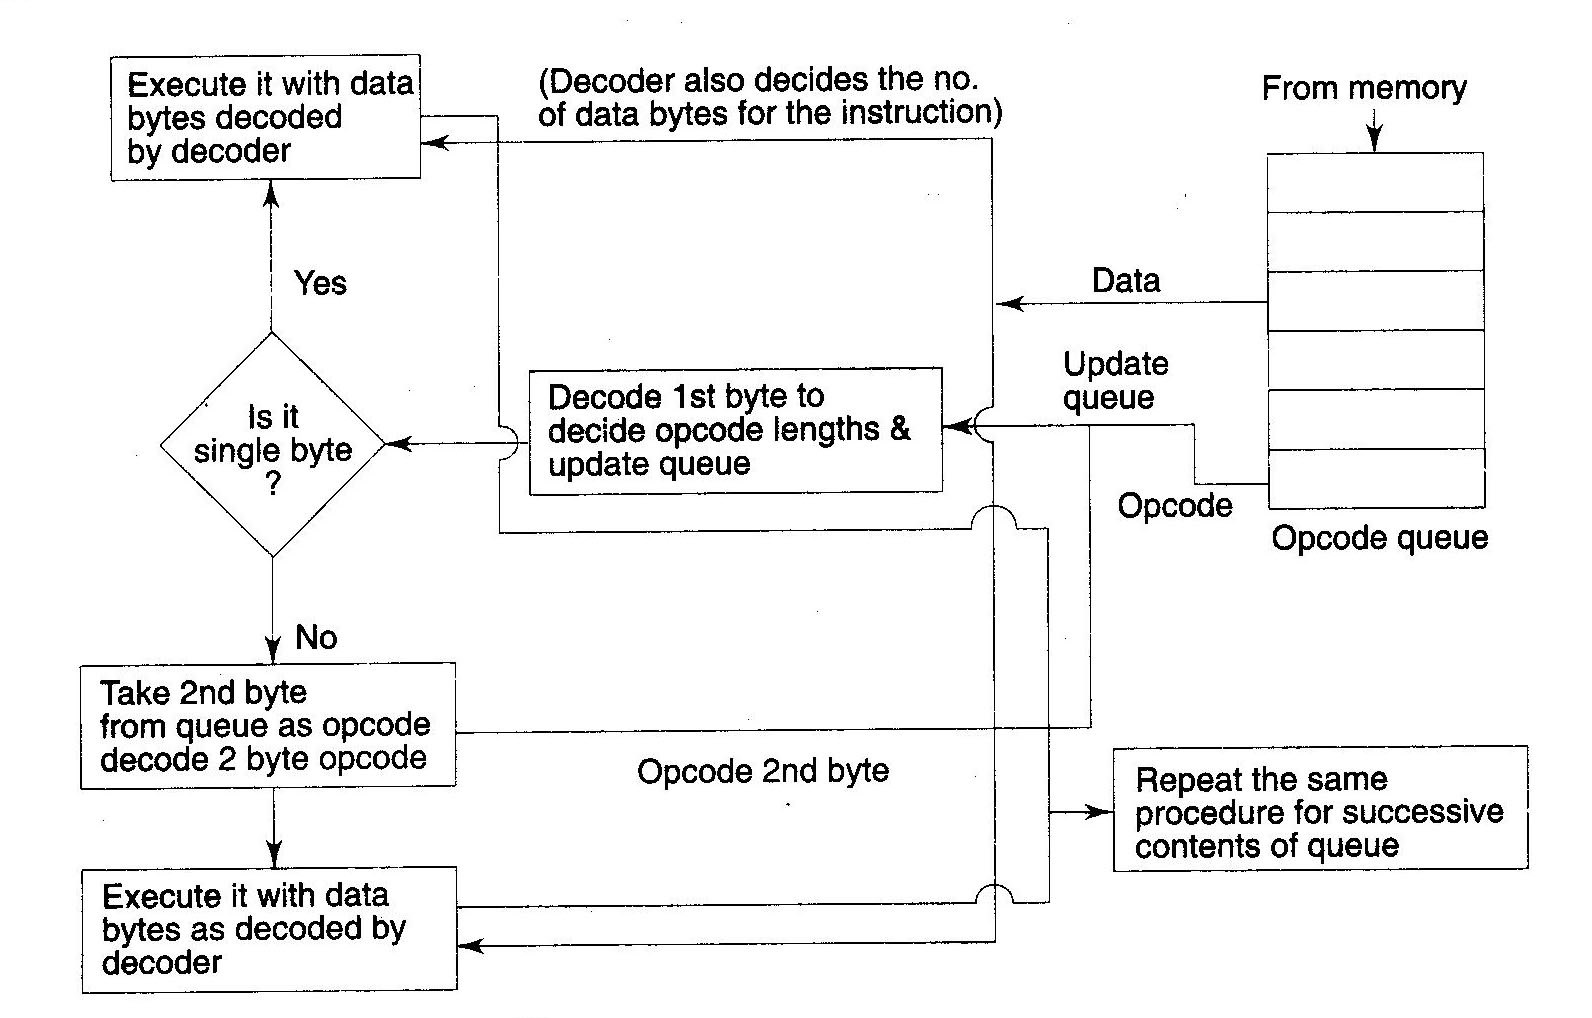
\includegraphics[width=0.89\textwidth]{images/8086-instruction-queue-operation.png}
		\caption{8086 General instruction queue operation flow chart.}
		\label{image-16}
	\end{figure}
	
	\textbf{Program segments: }Program's code, data, and stack are loaded into different memory segments, namely code segment, data segment, and stack segment. At any time, only four memory segments are active. A program segment need not occupy the entire 64 KB. Data segment contains variable declarations and is declared by .DATA. Stack segment is used to store the stack, and is declared by .STACK size. Default size of stack is 1 KB. A code segment contains the program's instructions, and is declared by .CODE.\\
	
	\textbf{Memory Models: }Following are memory models in 8086:\\
	
	SMALL: Code in one segment, and data in one segment.\\
	
	MEDIUM: Code in more than one segment, and data in one segment.\\
	
	COMPACT: Code in one segment, and data in more than one segment.\\
	
	LARGE: Code in more than one segment, and data in more than one segment, and no array 
	larger than 64 KB.\\
	
	HUGE: Code in more than one segment, and data in more than one segment, and arrays may be larger than 64 KB.
	
\section{Most asked Assembly Language Programs (ALPs)} Roughly ordered in increasing order of difficulty. One program may ask for writing more than one assembly programs.
	\begin{enumerate}
		\item Write assembly language programs (ALPs) for addition and subtraction of n numbers (16 bits and 32 bits).
		\item Write assembly language programs (ALPs) for multiplication and division of n numbers (16 bits and 32 bits). 
		\item Write assembly language programs (ALPs) to determine GCD (HCF) and LCM of two numbers (16-bits and 32 bits). 
		\item Write an assembly language program (ALP) to evaluate expressions. 
		\item Write assembly language programs (ALPs) for sorting and searching (Finding maximum and minimum numbers among n numbers). 
		\item Write assembly language programs (ALP) to perform Shift and rotate operations. 
		\item Write an assembly language program (ALP) to check whether given data is positive or negative using bit manipulation instructions.
		\item Write an assembly language program (ALP) to count number of 0s and 1s in a given data.
		\item Write an assembly language program (ALP) to check bit wise and nibble wise palindrome.
		\item Write an assembly language program (ALP) for converting packed BCD to unpacked BCD. 
		\item Write an assembly language program (ALP) for BCD to ASCII conversion (Using arithmetic and logical instructions).  
		\item Write an assembly language program (ALP) for moving a block of data from one memory location to another.
		\item Write an assembly language program (ALP) for reversing a string.
		\item Write an assembly language program (ALP) for comparison of two strings.
		\item Write an assembly language program (ALP) to find length of a string using string instructions.
		\item Write an assembly language program (ALP) to change an already available ascending order byte string to descending order.
		\item Write an assembly language program (ALP) to convert a given sixteen bit binary number to its GRAY equivalent.
		\item Write an assembly language program (ALP) to find out transpose of a 3x3 matrix.
		\item Write an assembly language program (ALP) to find nth Fibonacci number.
		\item Write an assembly language (ALP) program for separation of odd and even numbers.
		\item Write an assembly language program (ALP) to find out cube (or square) of an 8-bit hexadecimal number.
		\item Write an assembly language program (ALP) for traffic light controller.
	\end{enumerate}
\section{Question Bank}
	\begin{enumerate}
		\item What is Pipelining and Segmentation? What were the drawbacks of 8085 that were overcame by them. What is the use of memory segmentation in 8086?
		\item Which pins determine the mode of operation of 8086? What are the pins that specify various types of transfer in minimum and maximum mode?
		\item What are the types of transfer of 8086? What is the use of Bus controller?
		\item Explain in brief following terms: Bus, Memory module, I/O subsystem, Interface, Memory Interface, I/O Interface.
		\item Explain the internal architecture of 8086 with diagram.
		\item Describe the functions of EU and BIU.
		\item Explain register organization of 8086. What the function of various registers and pointers in 8086?
		\item Describe Flag register with its functions in 8086
		\item How 20-bit address is generated in 8086?
		\item Explain timing diagrams of memory read and memory write machine cycles in 8086.
		\item Explain minimum and maximum mode of 8086? Which mode is used for multiprocessor configuration?
		\item What are various flags of 8086?
		\item What are operators and operands? 
		\item Enlist various instructions of 8086?
		\item Describe following instructions: Data transfer instructions, Arithmetic instructions, Bit manipulation instructions, Program control instructions, Processor control instructions, string instructions.
		\item What are addressing modes? Explain various addressing modes in 8086?
		\item What are Procedures and MACROS? Write functions of them. 
		\item What are the differences between procedures and MACROS? What is the fundamental difference between a MACRO and a subroutine? Enlist various advantages and disadvantages of Macros.
		\item Explain various machine language instruction formats supported by 8086.
		\item What is Assembler and linker? What are the differences between them?
		\item What are interrupts? Describe functions of an interrupt vector table. How many interrupts are there in 8085. Explain their maskability property and priority order between them.
		\item What are the procedures when interrupt happens in 8086. 
		\item How are stack pointer and stack segment registers initialized when pushing first element on to a stack?
		\item Describe interrupts. Classify vectored and non-vectored interrupts in 8086. Write a simple routine to demonstrate software interrupt procedure.
	\end{enumerate}
\end{document}
